\section{Hermite cubics}
\label{sec:Hermite cubics}

In order to have $C^1$ global interpolator we need to select a different basis.

\paragraph{Hermite cubics in $(0,1)$}
Let us take $K = (0,1)$.
We take $\mathcal P = \mathbb R_3[x]$.
We pick as nodal functions
\begin{equation*}
    N_1 (v) = v(0), \qquad N_2(v) = v(1), \qquad N_3(v) = \frac{dv}{dx} (0), \qquad N_4(v) = \frac{dv}{dx} (1).
\end{equation*}
Our nodal basis will be $\theta_0, \cdots, \theta_3$ such that
\begin{equation*}
    \begin{matrix}
        \theta_0(0) = 1, & \theta_0(1) = 0, & \theta_0'(0) = 0, & \theta_0'(1) = 0
        \\
        \theta_1(0) = 0, & \theta_1(1) = 1, & \theta_1'(0) = 0, & \theta_1'(1) = 0
        \\
        \theta_2(0) = 0, & \theta_2(1) = 0, & \theta_2'(0) =1,  & \theta_2'(1) = 0
        \\
        \theta_3(0) = 0, & \theta_3(1) = 0, & \theta_3'(0) =0,  & \theta_3'(1) = 1
    \end{matrix}
\end{equation*}
Solving for the exact values leads to \eqref{fig:Hermite cubic nodal basis}
\begin{figure}[H]
    \centering
    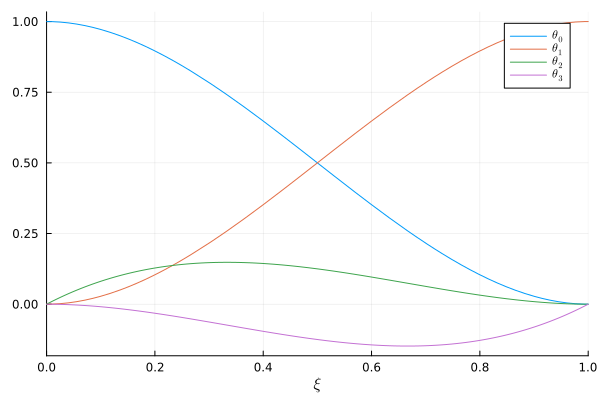
\includegraphics[width=.5\textwidth]{Hermite_reference_element.png}
    \caption{Nodal basis for the Hermite cubics}
    \label{fig:Hermite cubic nodal basis}
\end{figure}

The local interpolator is given by
\begin{equation*}
    \mathcal I_{K} v (x) = v(0) \theta_0(x) + v(1) \theta_1(x) + \frac{dv}{dx} (0) \theta_2 (x) + \frac{dv}{dx} (1) \theta_3 (x).
\end{equation*}

\paragraph{Hermite cubics on $(a,b)$}
Due to \Cref{rem:FEM affine equivalence element with derivatives} we will not apply \Cref{thm:FEM affine equivalence and interpolation estimate}, so we perform the estimate in a generic interval.

Let us take $K = (a,b)$.
We take $\mathcal P = \mathbb R_3[x]$.
We pick as nodal functions
\begin{equation*}
    N_1 (v) = v(a), \qquad N_2(v) = v(b), \qquad N_3(v) = \frac{dv}{dx} (a), \qquad N_4(v) = \frac{dv}{dx} (b).
\end{equation*}
Discuss in \Cref{ex:FEM affine equivalence Hermite cubics} this is not affine equivalent to the element in $(0,1)$. However, the shape functions are
\begin{equation*}
    \psi_1(x) = \theta_0 (\tfrac{x-a}{b-a}), \qquad \psi_2(x) = \theta_1 (\tfrac{x-a}{b-a}), \qquad \psi_3(x) = (b-a) \theta_2 (\tfrac{x-a}{b-a}), \qquad \psi_4(x) = (b-a) \theta_3 (\tfrac{x-a}{b-a})
\end{equation*}

\paragraph{Local interpolation in an interval $K$}
In dimension $d=1$ we have that $\rho_K = h_K$.
We can use \Cref{thm:FEM bound interpolation error} to deduce that
\begin{equation*}
    [v - \mathcal I_K v]_{W^{j,p} (K)} \le C h_K^{4-j}[v]_{W^{4,p}(K)}, \qquad j \in \{0, \cdots, 4\}.
\end{equation*}


\paragraph{$H^2$-global interpolation}
Since our local interpolator preserves the value of the function and its derivative at $x=0$ and $x=1$ we can build a basis of $\mathcal P_{\mathcal T} \cap H^2(a,b)$ non-trivial.
Hence, given a domain $\Omega = (a,b)$ and sub-division $\mathcal T$ made on intervals, the global interpolator will yield
$$
    \mathcal I_{\mathcal T} : C^1( [a,b] ) \to \mathcal C^1([a,b]), \qquad \mathcal I_{\mathcal T} : H^2(a,b) \to H^2(a,b).
$$
Let us take a sub-division of $(a,b)$ of the form $x_0 = a, \cdots, x_N = b$. Let us describe the finite-element space generate by using Hermite cubics in each interval to generate $C^1$ functions. To this end, we build a basis made out of $v_i$ and $w_i$.
We have to properly ``glue'' by setting
$$
    v_{i}(x_j) = \delta_{ij}, \qquad v'_i (x_j) = 0, \qquad w_i (x_j) = 0, \qquad w_i'(x_j) = \delta_{ij}
$$
This leads to the basis elements $\varphi_{2i} = v_i$ and $\varphi_{2i + 1} = w_i$ with
$$
    v_{i} (x) =
    \begin{cases}
        \theta_1 \left( \frac{x-x_{i-1}}{x_{i}-x_{i-1}} \right) , & x \in [x_{i-1},x_{i}) \\
        \theta_0 (\frac{x-x_{i}}{x_{i+1}-x_{i}}) ,                & x \in [x_{i},x_{i+1}) \\
        0,                                                        & \text{otherwise},
    \end{cases}
    \qquad
    w_{i} (x) =
    \begin{cases}
        (x_{i}-x_{i-1}) \theta_4 \left( \frac{x-x_{i-1}}{x_{i}-x_{i-1}} \right) , & x \in [x_{i-1},x_{i})       \\
        (x_{i+1}-x_{i}) \theta_3 (\frac{x-x_{i}}{x_{i+1}-x_{i}}) ,                & x \in x \in [x_{i},x_{i+1}) \\
        0,                                                                        & \text{otherwise}.
    \end{cases}
$$
See \Cref{fig:Hermite cubics basis functions}.
Then we have the interpolant
\begin{equation*}
    \mathcal I_{\mathcal T} u(x) = \sum_{i=0}^N \Big( u(x_j) v_i(x) + \frac{du}{dx}(x_j) w_i (x)\Big).
\end{equation*}
Notice that $\mathcal I_{\mathcal T} u(x_j) = u(x_j)$ and $\frac{d \mathcal I_{\mathcal T} u}{dx} (x_j) = \frac{du}{dx}(x_j)$ for all points in the mesh.


\begin{figure}[H]
    \centering
    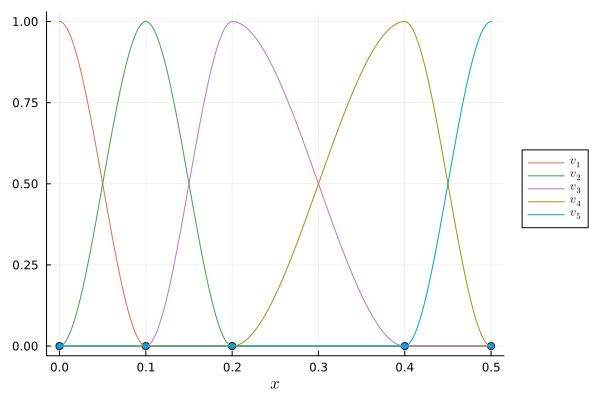
\includegraphics[width=.45\textwidth]{Hermite_interval_v.png}
    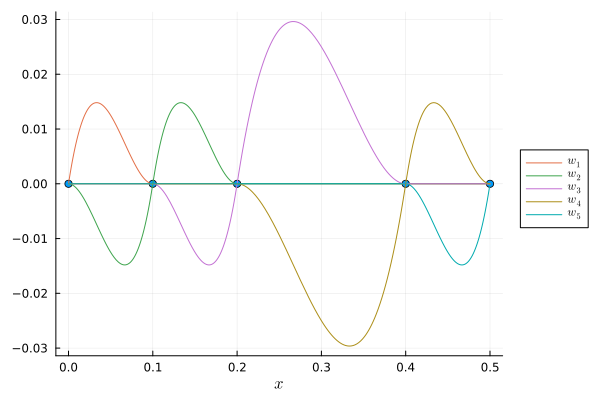
\includegraphics[width=.45\textwidth]{Hermite_interval_w.png}
    \caption{$C^1$-basis functions on a sub-division of $(0,0.5)$ based on Hermite cubics}
    \label{fig:Hermite cubics basis functions}
\end{figure}

\begin{remark}
    If we only want to build a basis of $\mathcal P_{\mathcal T} \cap H^1(a,b)$ we would take the basis of $\mathcal P_{\mathcal T} \cap H^2(a,b)$ and add the elements $z_i$ made by glueing $\theta_3$s and $\theta_4$s with discontinuity in the derivative.
    This is a highly unnatural and unpleasant task that we will not undertake.
    
    This is not a good idea since the point of moving to this basis is approximating $u$ that is very regular.
    If $u$ is not $C^1$ then we cannot use $I_\mathcal T$. If $u$ is $C^1$ regular then $I_{\mathcal T} u \in \mathcal P_{\mathcal T} \cap C^1(a,b)$. 
    And we want $u$ to be more than $C^1$ regular in order to get any rates.
\end{remark}

\paragraph{$H^2$-global-interpolation error}
Notice that due to the $C^1$-glueing, the interpolant is at most $H^2$.
We have for $j \in \{0, 1, 2\}$ that
\begin{align*}
    [v - \mathcal I_K v]_{H^j (a,b)}
     & = \left( [v - \mathcal I_K v]_{H^j (a,b)}^2 \right)^{\frac 1 2}
    = \left( \sum_{i=1}^N [v - \mathcal I_K v]_{H^j (x_{i-1},x_i)}^2 \right)^{\frac 1 2}
    \\
     & \le \left( C \sum_{i=1}^N (x_{i} - x_{i-1})^{2(4-j)} [v]_{H^4 (x_{i-1},x_{i})}^2 \right)^{\frac 1 2} \\
     & \le C h_{\mathcal T}^{4-j}[v]_{H^4 (a,b)}.
\end{align*}
Using Céa's lemma in \Cref{ex:Galerkin Laplace piecewise linear Cea} we use $H^1$ estimates and a convergence rate up to $h_{\mathcal T}^3$.